\let\negmedspace\undefined
\let\negthickspace\undefined
\documentclass[journal,12pt,onecolumn]{IEEEtran}
\usepackage{cite}
\usepackage{amsmath,amssymb,amsfonts,amsthm}
\usepackage{algorithmic}
\usepackage{graphicx}
\graphicspath{{./figs/}}
\usepackage{textcomp}
\usepackage{xcolor}
\usepackage{txfonts}
\usepackage{listings}
\usepackage{enumitem}
\usepackage{mathtools}
\usepackage{gensymb}
\usepackage{comment}
\usepackage{caption}
\usepackage[breaklinks=true]{hyperref}
\usepackage{tkz-euclide} 
\usepackage{listings}
\usepackage{gvv}                                        
%\def\inputGnumericTable{}                                 
\usepackage[latin1]{inputenc}     
\usepackage{xparse}
\usepackage{color}                                            
\usepackage{array}
\usepackage{longtable}                                       
\usepackage{calc}                                             
\usepackage{multirow}
\usepackage{multicol}
\usepackage{hhline}                                           
\usepackage{ifthen}                                           
\usepackage{lscape}
\usepackage{tabularx}
\usepackage{array}
\usepackage{float}
\newtheorem{theorem}{Theorem}[section]
\newtheorem{problem}{Problem}
\newtheorem{proposition}{Proposition}[section]
\newtheorem{lemma}{Lemma}[section]
\newtheorem{corollary}[theorem]{Corollary}
\newtheorem{example}{Example}[section]
\newtheorem{definition}[problem]{Definition}
\newcommand{\BEQA}{\begin{eqnarray}}
\newcommand{\EEQA}{\end{eqnarray}}
\newcommand{\define}{\stackrel{\triangle}{=}}
\theoremstyle{remark}
\newtheorem{rem}{Remark}

\begin{document}

\title{2.10.84}
\author{ee25btech11056 - Suraj.N}
\maketitle
\renewcommand{\thefigure}{\theenumi}
\renewcommand{\thetable}{\theenumi}

\begin{document}

\textbf{Question :} Let $Q$ be the cube with the set of vertices 
\[
\{(x_1, x_2, x_3) \mid x_1, x_2, x_3 \in \{0,1\}\} \subset \mathbb{R}^3
\]
Let $F$ be the set of all twelve lines containing the diagonals of the six faces of the cube $Q$.  
Let $S$ be the set of all four lines containing the main diagonals of the cube $Q$; for instance, the line passing through the vertices $(0,0,0)$ and $(1,1,1)$ is in $S$.  

For lines $\lambda_1$ and $\lambda_2$, let $d(\lambda_1, \lambda_2)$ denote the shortest distance between them.  
Then the maximum value of $d(\lambda_1, \lambda_2)$, as $\lambda_1$ varies over $F$ and $\lambda_2$ varies over $S$, is\\\\ 

\textbf{Solution :} the diagonals of the cube can be written as 

\begin{table}[h!]
  \centering
  \begin{tabular}{|c|c|}
\hline
Line & Equation \\
\hline
Body diagonal & $\vec{x} = \myvec{0\\0\\1} + k_1\myvec{1\\1\\-1}$ \\
\hline
Face diagonal & $\vec{x} = \myvec{0\\0\\0} + k_2\myvec{1\\0\\1}$ \\
\hline
\end{tabular}


  \caption*{Table : diagonals}
  \label{2.10.84}
\end{table}

\begin{align}
\vec{x} &= \vec{A} + k_1\vec{m}_1, \quad \vec{A} = \myvec{0\\0\\1}, \; \vec{m}_1 = \myvec{1\\1\\-1} \\
\vec{x} &= \vec{B} + k_2\vec{m}_2, \quad \vec{B} = \myvec{0\\0\\0}, \; \vec{m}_2 = \myvec{1\\0\\1}
\end{align}

\begin{align}
\vec{M} = \myvec{\vec{m_1} & \vec{m_2}} = \myvec{1 & 1 \\1 & 0 \\-1 & 1}
\end{align}

\begin{align}
  \myvec{\vec{B} - \vec{A}} = \myvec{0\\0\\-1}
\end{align}


\begin{align}
\myvec{\vec{M} & \vec{B}-\vec{A}} = \myvec{1 & 1 & 0 \\1 & 0 & 0 \\-1 & 1 & -1}
\end{align}

Performing row operations:
\begin{align}
    \myvec{
        1 & 1 & 0 \\[6pt]
        1 & 0 & 0 \\[6pt]
       -1 & 1 & -1
    }
    &\xleftrightarrow{R_2 \to R_2 - R_1}
    \myvec{
        1 & 1 & 0 \\[6pt]
        0 & -1 & 0 \\[6pt]
       -1 & 1 & -1
    }
   \xleftrightarrow{R_3 \to R_3 + R_1}
    \myvec{
        1 & 1 & 0 \\[6pt]
        0 & -1 & 0 \\[6pt]
        0 & 2 & -1
    }
    \xleftrightarrow{R_3 \to R_3 + 2R_2}
    \myvec{
        1 & 1 & 0 \\[6pt]
        0 & -1 & 0 \\[6pt]
        0 & 0 & -1
    }
\end{align}

Clearly, the rank of this matrix is 3, and therefore, the lines are skew.

\pagebreak

From the least squares formulation,  
\begin{align}
  \vec{M}^\top\vec{M}\myvec{k_1 \\ -k_2} &= \vec{M}^\top\myvec{\vec{B}-\vec{A}}
\end{align}

Thus,
\begin{align}
\vec{M}^\top\vec{M} &= 
\myvec{
1 & 1 & -1 \\
1 & 0 & 1
}
\myvec{
1 & 1 \\
1 & 0 \\
-1 & 1
} = \myvec{3 & 0 \\ 0 & 2} \\
\vec{M}^\top(\vec{B}-\vec{A}) &= 
\myvec{1 & 1 & -1 \\ 1 & 0 & 1}
\myvec{0\\0\\-1} 
= \myvec{1 \\ -1}
\end{align}

Therefore,
\begin{align}
\myvec{3 & 0 \\ 0 & 2}
\myvec{k_1 \\ -k_2}
= \myvec{1\\-1}.
\end{align}

Solving,

\begin{align}
  \myvec{k_1\\-k_2} = \myvec{\frac{1}{3} \\[5pt] -\frac{1}{2}}
\end{align}

Hence the closest points are
\begin{align}
\vec{P} &= \vec{A} + k_1\vec{m}_1 
= \myvec{0\\0\\1} + \tfrac{1}{3}\myvec{1\\1\\-1}
= \myvec{\frac{1}{3}\\[5pt] \frac{1}{3}\\[5pt] \frac{2}{3}} \\
\vec{Q} &= \vec{B} + k_2\vec{m}_2 
= \myvec{0\\0\\0} + \tfrac{1}{2}\myvec{1\\0\\1}
= \myvec{\frac{1}{2}\\[5pt] 0\\[5pt] \tfrac{1}{2}}
\end{align}

The shortest distance is
\begin{align}
  \|\vec{P}-\vec{Q}\|
  = \left\|\myvec{-\frac{1}{6}\\[5pt] \tfrac{1}{3}\\[5pt] \tfrac{1}{6}}\right\| = \frac{1}{\sqrt{6}}
\end{align}

\pagebreak

\begin{figure}[h!]
  \centering
  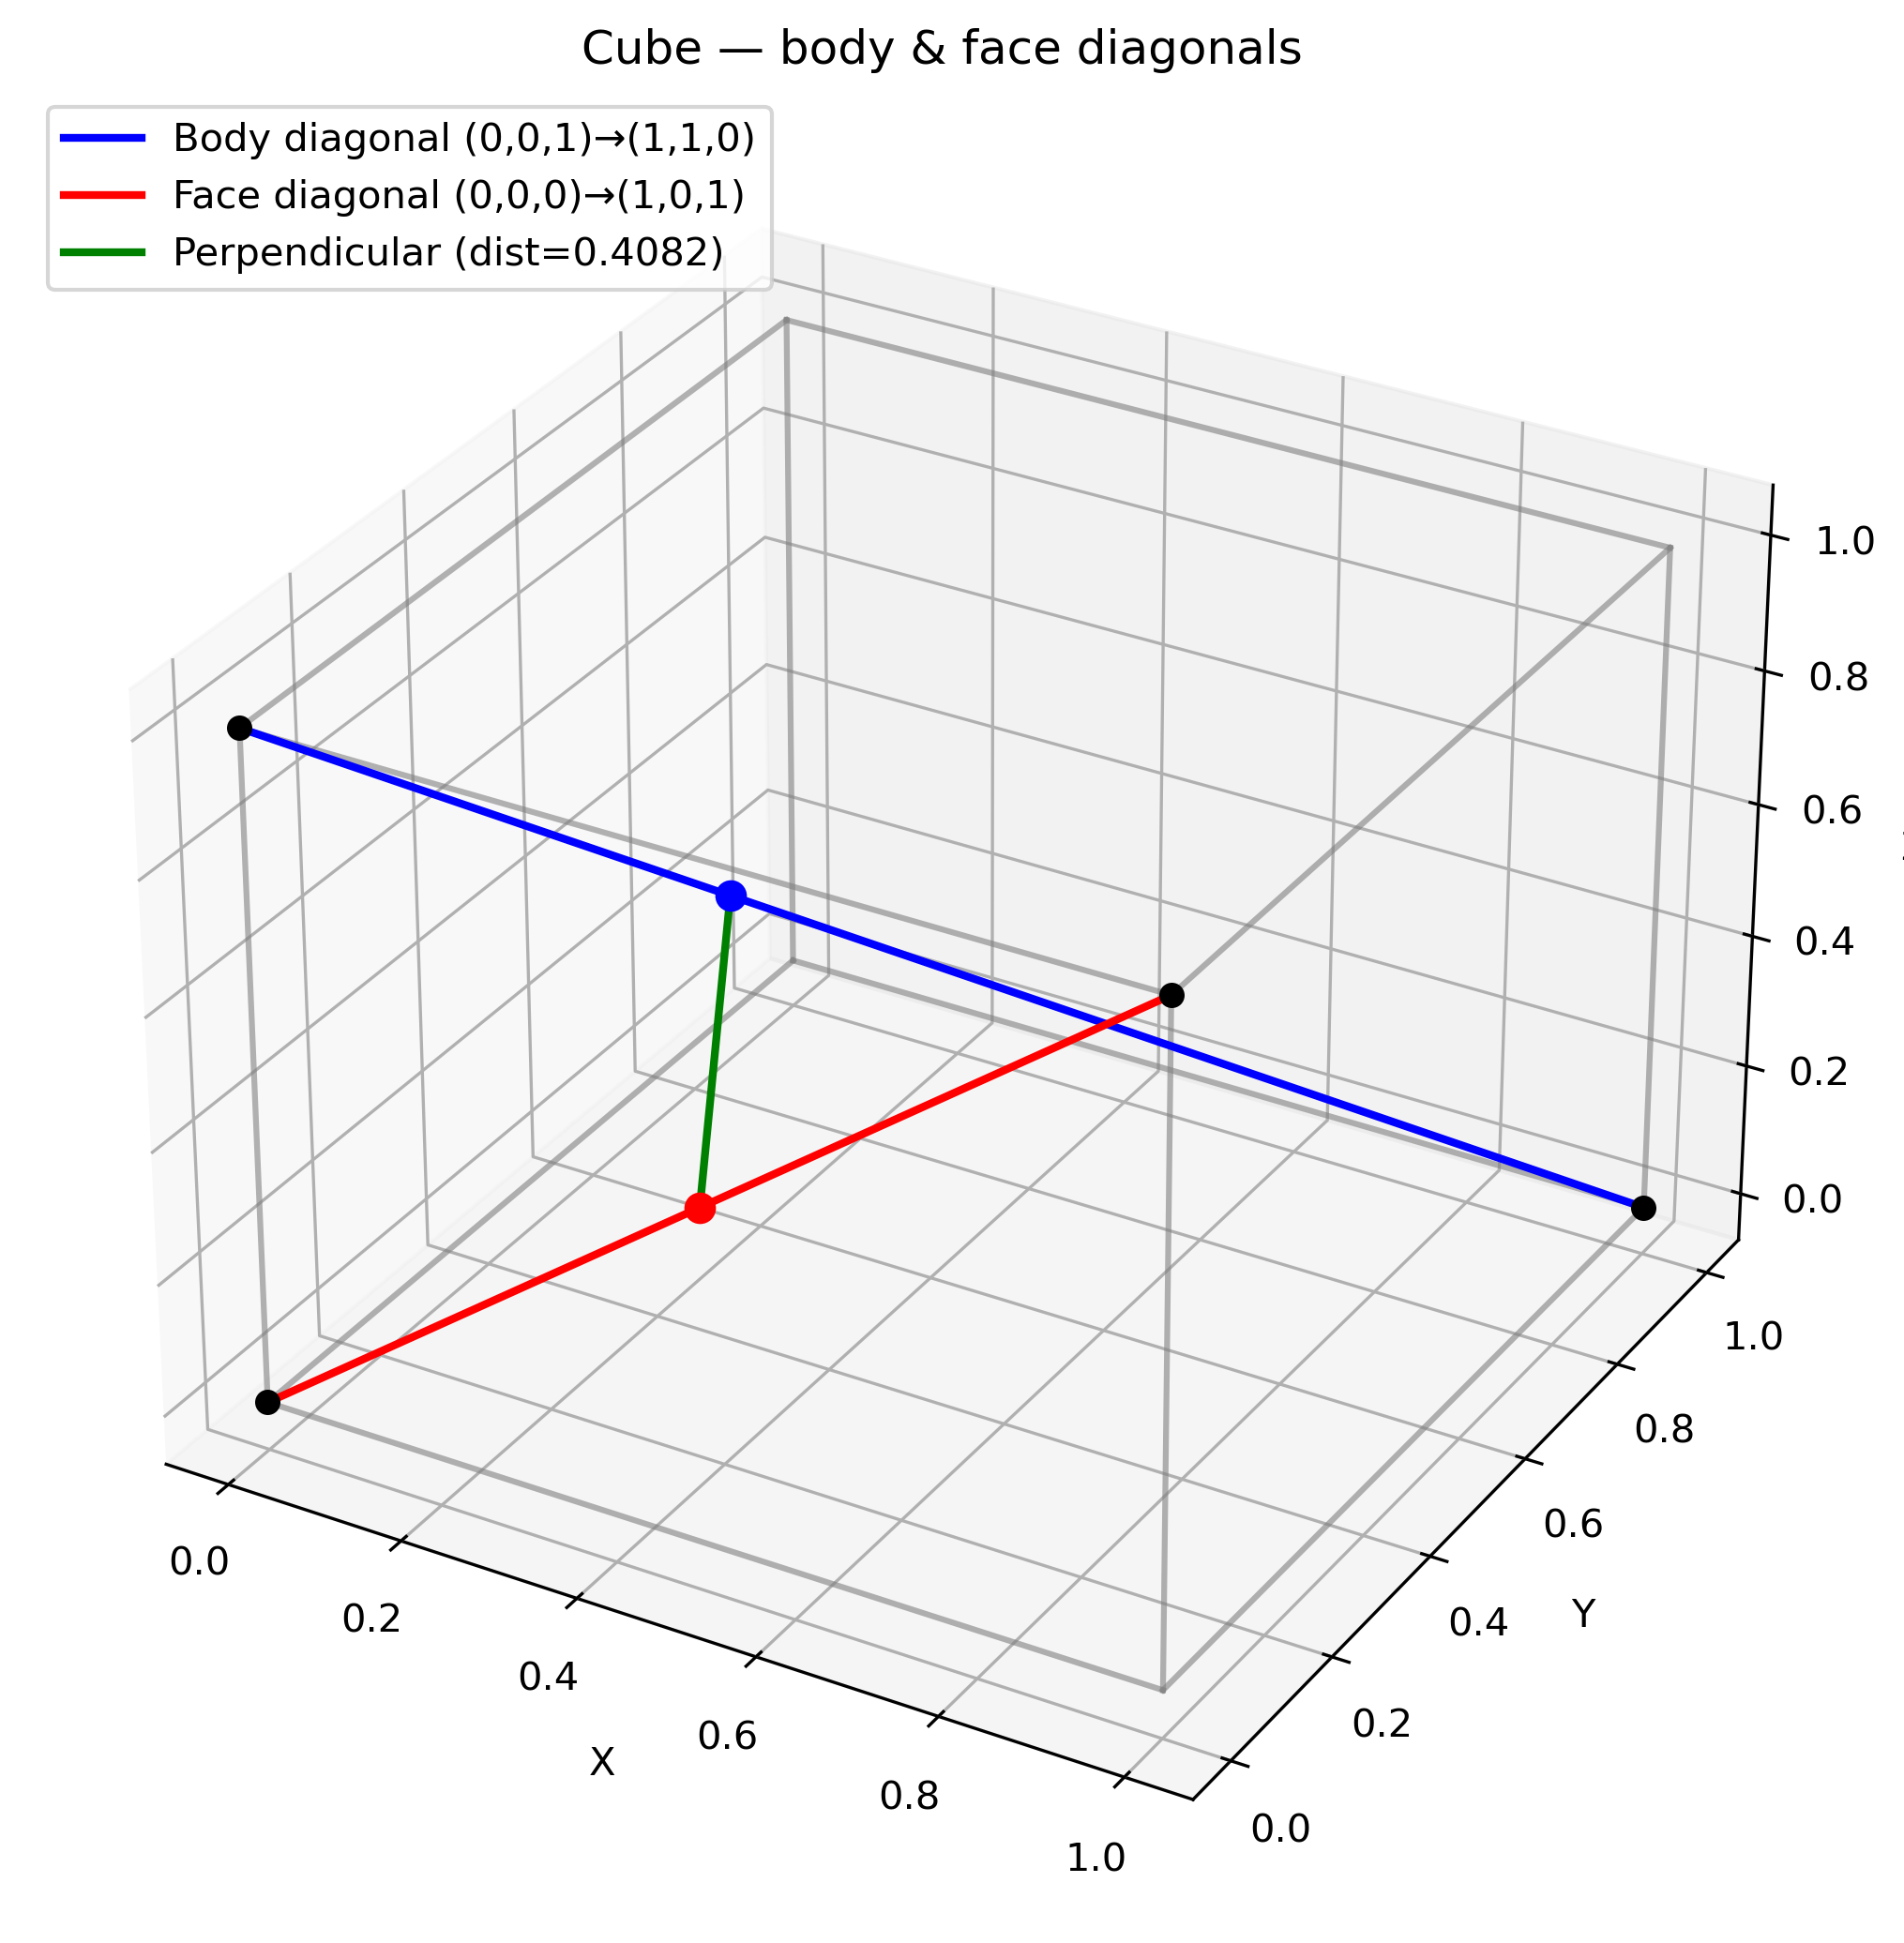
\includegraphics[width=0.7\columnwidth]{figs/cube_lines.png} 
   \caption*{Fig : diagonals}
  \label{Fig1}
\end{figure}



\end{document}
